\section{Production of $\Vzeros$ in Jets}

\subsection{Analysis strategy}

\subsubsection{Acceptance}\label{sec:c05DefAcc}

The details about the inclusive $\Vzeros$ analysis is described in
section~\ref{sec:c03InclusiveV0s}.
And the inclusive $\Vzeros$ are selected in $0<y_{\rm cms}<0.5$.
To match the $\Vzeros$ with the jets,
here we selected the $\Vzeros$ on $\eta-\phi$ plan
to get the uniform acceptance definition for both $\Vzeros$ and jets.

\begin{figure}[htb]
\begin{center}
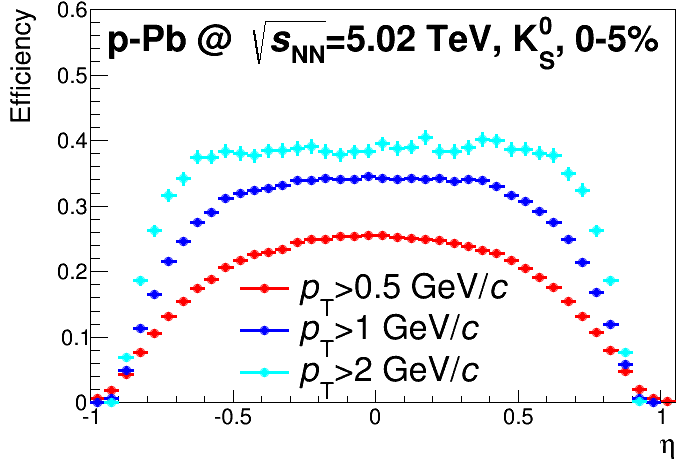
\includegraphics[width=.32\textwidth]{c05EffiV0Eta/cKshortEffiEta_000_005}
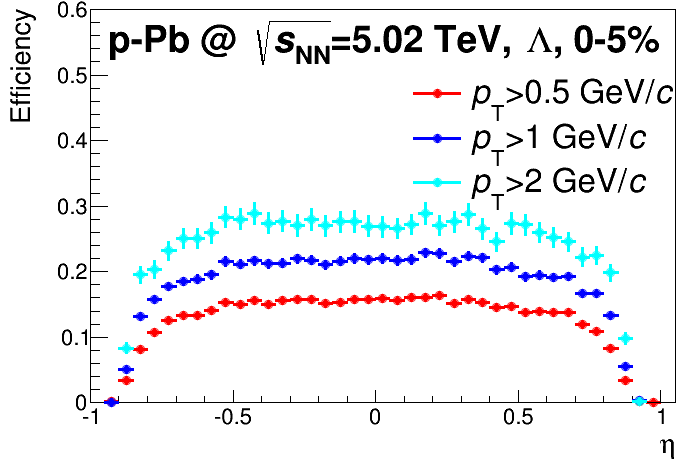
\includegraphics[width=.32\textwidth]{c05EffiV0Eta/cLambdaEffiEta_000_005}
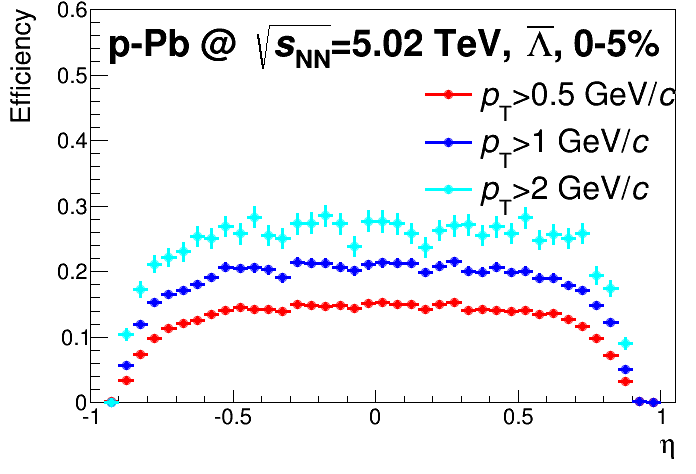
\includegraphics[width=.32\textwidth]{c05EffiV0Eta/cAntiLaEffiEta_000_005}
\caption{Efficiency of inclusive $\Vzeros$ as a function of $\eta$
         in central collisions ($0-5\%$, with V0A centrality estimator).}
\label{fig:c05EffiV0Eta000005}
\end{center}
\end{figure}

\begin{figure}[!htb]
\begin{center}
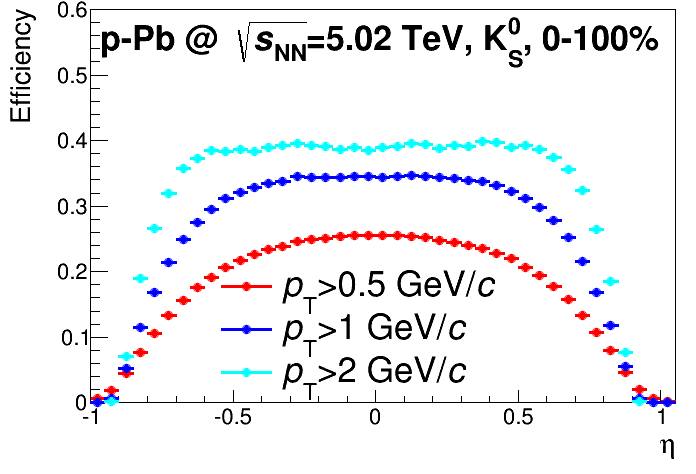
\includegraphics[width=.32\textwidth]{c05EffiV0Eta/cKshortEffiEta_000_100}
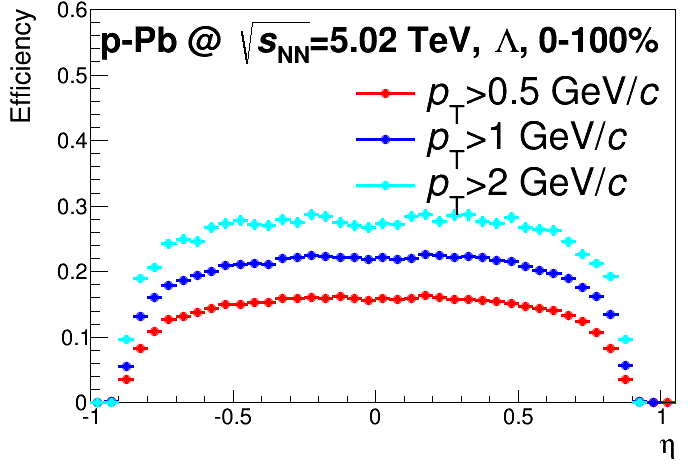
\includegraphics[width=.32\textwidth]{c05EffiV0Eta/cLambdaEffiEta_000_100}
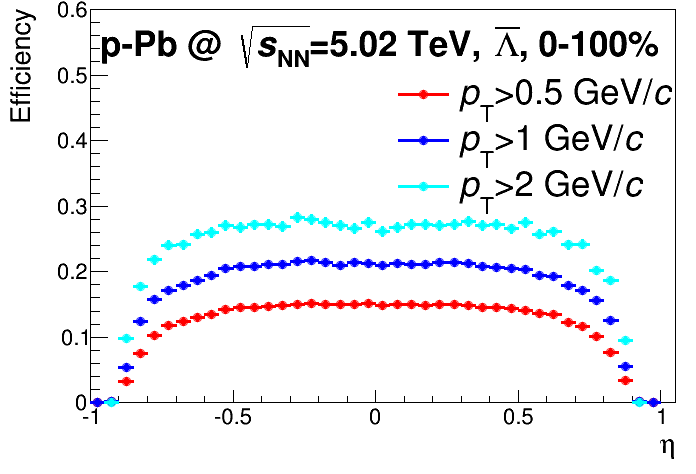
\includegraphics[width=.32\textwidth]{c05EffiV0Eta/cAntiLaEffiEta_000_100}
\caption{Efficiency of inclusive $\Vzeros$ as a function of $\eta$
         in MB event ($0-100\%$, with V0A centrality estimator).}
\label{fig:c05EffiV0Eta000100}
\end{center}
\end{figure}

Figure~\ref{fig:c05EffiV0Eta000005} and~\ref{fig:c05EffiV0Eta000100} shows
the efficiency of inclusive $\Vzeros$ as a function of $\eta$ in the central
collisions ($0-10\%$) and in MB events ($0-100\%$), respectively.
Due to the $\Vzero$ daughters are selected in $|\eta|<0.8$,
the efficiency is decreased when closing to this kinematics bound.
To minimize the bound effect on the $\Vzero$ candidates selection,
we restricted the $\Vzeros$ in and jets in:
\begin{itemize}
\item $\Vzeros$: $|\eta|<0.75$;
\item jets: $|\eta|<\eta_{\Vzero}^{\max}-R_{\rm jet}$ ($|\eta_{\rm jet}|<0.35$
      with $R_{\rm jet}=0.4$
      and $|\eta_{\rm jet}|<0.55$ with $R_{\rm jet}=0.2$).
\end{itemize}
The reducing of the jet acceptance is also useful to avoid the bound effect
in jet reconstruction.

\subsubsection{$\Vzero-$jet matching}
\label{sec:c05V0JetMat}

The first task to obtain the yield of $\Vzeros$ produced inside the jet cone
is to extract the number of $\Vzeros$ matched to the jets.
This is done with the following steps:
\begin{enumerate}
\item select the $\Vzero$ candidates with the cuts defined
      in section~\ref{sec:c03V0CandiSel},
      as discussed in section~\ref{sec:c05DefAcc},
      the $\Vzero$ candidates are selected in the acceptance of $|\eta|<0.75$;
\item match the $\Vzeros$ candidates and jets according to the geometry cut:
      \begin{equation}\label{eq:c05V0JetMatch}
      \Delta R_{\Vzero-{\rm jet}}<R_{\rm jet},
      \end{equation}
      where, $\Delta R_{\Vzero-{\rm jet}}$ is the distance between
      the $\Vzero$ and jet axis in $\eta-\phi$ plane;
\item fill the invariant mass distribution of the $\Vzero$ candidates
      matched to the jets in each $\Vzero$ $\pT$ bin, then define the signal
      window and the side bands of the filled invariant mass distribution
      according to the mean and width from the {\bf inclusive $\mathbf\Vzero$}
      invariant mass distribution;
\item fit the counts in the side bands and interpolate the result into the
      signal window;
\item the number of $\Vzeros$ matched to jets are obtained by subtracting
      the interpolated result from the counts in the signal window
      in each $\Vzero$ $\pT$ bin.
\end{enumerate}
The $\Vzeros$ (or $\Vzero$ candidates) which matched to the jets are named as
the {\bf JC $\mathbf\Vzeros$} (or {\bf JC $\mathbf\Vzero$ candidates}).

\begin{figure}[htb]
\begin{center}
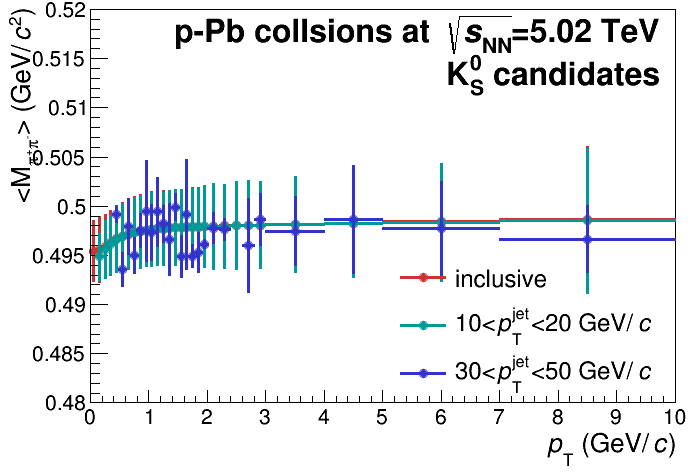
\includegraphics[width=.49\textwidth]{c05V0JetMat/KshortInvM}
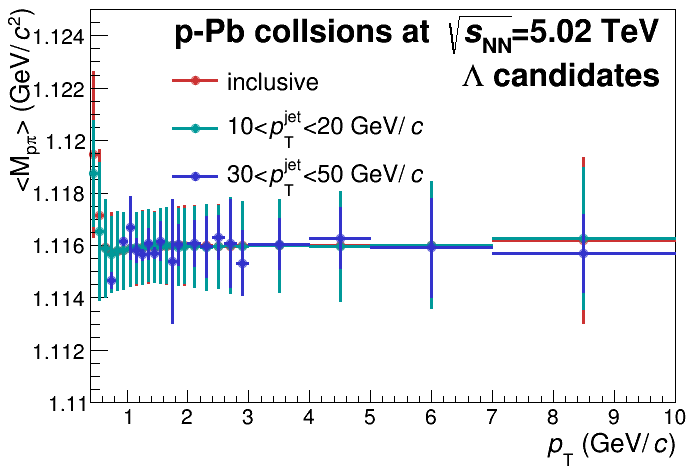
\includegraphics[width=.49\textwidth]{c05V0JetMat/LambdaInvM}
\caption{The mean and width of $\Vzero$ invariant mass distribution extracted
         by the Gaussian fit for the inclusive $\Vzeros$ candidates
         and JC $\Vzero$ candidates as a function of $\pT$ in data.}
\label{fig:c05CompV0FitInvM}
\end{center}
\end{figure}

Figure~\ref{fig:c05CompV0FitInvM} shows the comparison of the mean and width
of $\Vzero$ invariant mass distribution extracted by the Gaussian fit
for the inclusive $\Vzeros$ candidates and JC $\Vzero$ candidates
as a function of $\pT$ in data.
Indeed, the mean and width in the $\Vzero$ invariant mass distributions
for the inclusive $\Vzeros$ and JC $\Vzeros$ are almost the same.
But the large fluctuations caused by the less of the statistics are found
in these two variables obtained from the the JC $\Vzeros$ in the higher
jet $\pT$ bins.
To avoid these statistic fluctuations,
the number of JC $\Vzeros$ is extracted by using the mean and width
obtained in the inclusive $\Vzero$ invariant mass distribution.

Due to the $\Vzero$ candidates and the jets are reconstructed independently
in this analysis.
In eq.~(\ref{eq:c05V0JetMatch}) a $\Vzero$ candidate can match to
more than one jet due to the jet area is not always as a regular circle.
And this effect has to be considered when normalizing the JC
$\Vzeros$ to the corresponding number of
jets (see section~\ref{sec:c05NormV0s}).
To overcome the multiple countings in the normalization of
the JC $\Vzero$ sepectra,
the following steps are used for the $\Vzero-{\rm jet}$ matching:
\begin{itemize}
\item define a jet $\pT$ threshold, $\pT^{\min}$;
\item for a given $\Vzero$ candidate,
      made the loop over all the selected jets with $\pT$ above
      the $\pT^{\min}$ and in the corresponding jet $\eta$ acceptance
      in the event and,
      tagged it as the JC $\Vzero$ candidate if it can match with at least
      one selected jet in the event according to eq.~(\ref{eq:c05V0JetMatch}).
\end{itemize}

\subsubsection{Underlying $\Vzero$ estimation}
\label{sec:c05EstiV0sUE}

To obtain the spectra of $\Vzeros$ produced in the jets,
the $\Vzeros$ produced in the underlying events ({\bf UE $\mathbf\Vzeros$})
have to be subtracted from the yield of JC $\Vzeros$.
The basic idea is to use the $\Vzeros$ outside the jet cone to estimate
the density of the UE $\Vzeros$ inside jet cone.
But there are two effects which bias the underlying $\Vzero$ evaluation:
\begin{itemize}
\item the $\Vzeros$ outside the selected jets could be
      matched with the excluded jets which are rejected by
      the $\pT$ and $\eta$ cuts of the jet selection;
\item due to the detector response and the jet reconstruction efficiency,
      the physical jets associated to the $\Vzeros$ could be lost by the
      jet finder.
\end{itemize}

In this case, we use two different methods to estimate underlying $\Vzeros$:
\begin{itemize}
\item $\Vzeros$ outside jet cone ({\bf OC $\mathbf\Vzeros$}):
      \begin{equation}\label{eq:c05OCV0s}
      \Delta R_{\Vzero-{\rm jet}}>R_{\rm cut},
      \end{equation}
      where, $R_{\rm cut}$ is a given threshold of the distance between the
      $\Vzero$ and jet axis in $\eta-\phi$ plane;
\item $\Vzeros$ in events without any selected jet ({\bf NJ $\mathbf\Vzeros$}).
\end{itemize}

According to the definitoin,
the OC $\Vzeros$ are selected in the same event sample as the JC $\Vzeros$
and they can include both the $\Vzeros$ in the excluded jets and
the physical jets lost by the jet finder,
they have a strong correlation to the $\Vzeros$ produced in the jets.
On the other hand, if the $\pT$ threshold used to select the jet is low enough,
we do not expect there would be a strong hard scattering in the NJ events,
and the probability for the NJ $\Vzeros$ to match to the physical jets
is lower and their correlations to the $\Vzeros$ produced in the jets
is weaker.

In this analysis,
the JC $\Vzeros$ and the OC $\Vzeros$ are selected in the two open
jet $\pT$ bins: $\pT^{\rm jet}>10~\GeVc$ and $\pT^{\rm jet}>20~\GeVc$.
The {\bf corrected} jet $\pT$ in eq.~(\ref{eq:c04DefEstiJetPT}) is used
for the jet selection.
The NJ $\Vzeros$ are defined in the event without jet
in {\bf measured} $\pT>5~\GeVc$.
The uncertainly on UE $\Vzero$ estimation is given by the
difference between the OC and NJ $\Vzeros$.

\subsection{Efficiency}

\subsubsection{$\Vzero$ efficiency in MC}
\label{sec:c05V0EffiMC}

\begin{figure}[htb]
\begin{center}
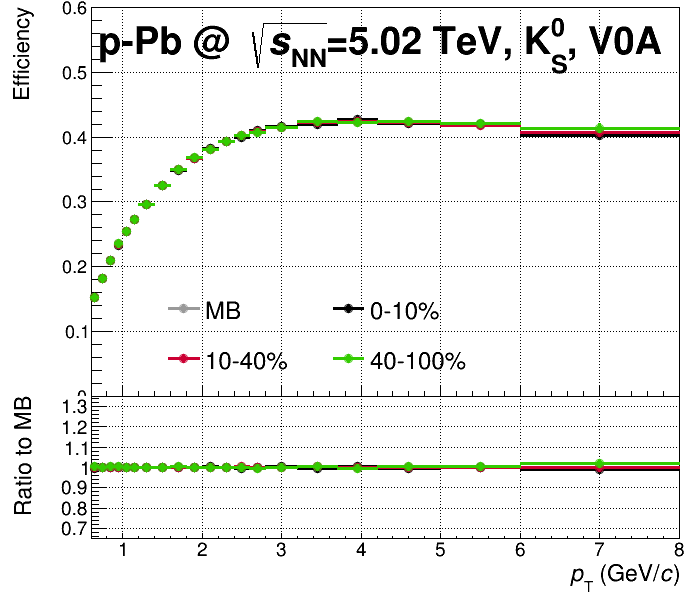
\includegraphics[width=.32\textwidth]{c05EffIncV0s/cKshort_Efficiency}
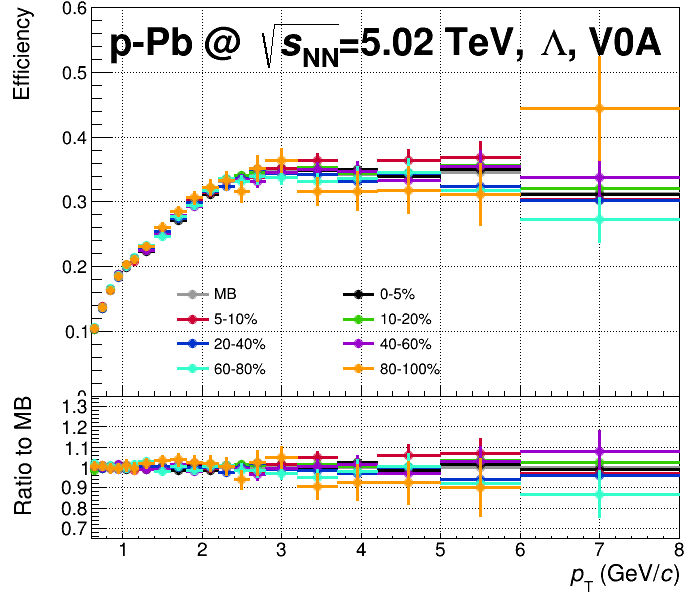
\includegraphics[width=.32\textwidth]{c05EffIncV0s/cLambda_Efficiency}
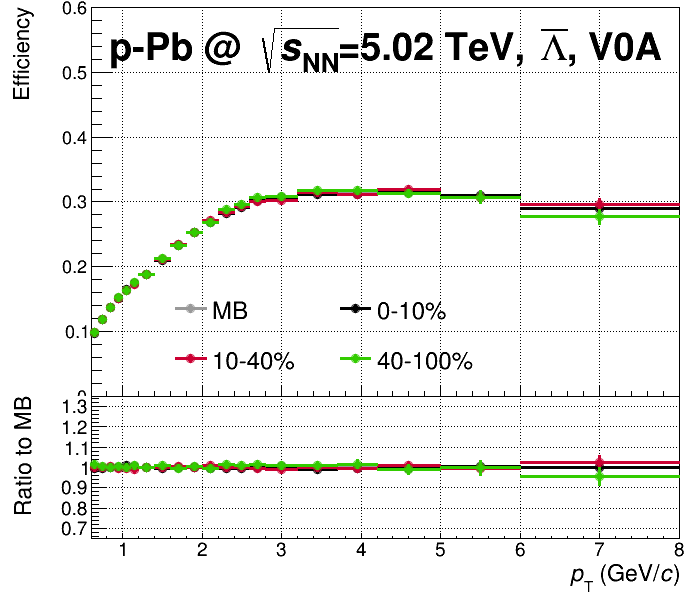
\includegraphics[width=.32\textwidth]{c05EffIncV0s/cAntiLa_Efficiency}
\caption{Efficiency of inclusive $\Vzeros$ as a function of $\pT$
         in three event multiplicity bins with V0A centrality estimator.}
\label{fig:c05EffiIncV0s}
\end{center}
\end{figure}

Figure~\ref{fig:c05EffiIncV0s} shows the efficiency of the inclusive $\Vzeros$
as a function of $\pT$ in three event multiplicity bins.
The results are obtained with the strategy introduced
in section~\ref{sec:c03AnaStrategy}.
The ratio of the efficiency in each event multiplicity bins and that in the
minimum-bias events ($0-100\%$) is also presented in this figure.
One can find that, the efficiency of inclusive $\Vzeros$ is independent on
the event multiplicity.

To implement the efficiency correction to the JC and OC $\Vzeros$ one has to
consider that,
the efficiency of $\Vzeros$ inside and outside jet cone could be different.
As a testing, we used to the following steps to check the efficiency of
JC $\Vzeros$
in the simulations:
\begin{enumerate}
\item reconstruct and select the jets in the simulations at
      detector level (with the reconstructed tracks) with the same criteria
      as in data,
\item match the physical primary $\Vzeros$ at particle level (the generated
      particles) to the reconstructed jets to build the denominator of
      the efficiency;
\item reproduce the steps in section~\ref{sec:c05V0JetMat} to obtain the
      number of JC $\Vzeros$ at detector level and use it to build the
      numerator of the efficiency.
\end{enumerate}
This procedure is summarized
in~\cite{Zimmermann:AliPWGJE20140401}~\footnote{There are two strategies for
the efficiency estimation of JC $\Vzeros$  in MC are proposed
in~\cite{Zimmermann:AliPWGJE20140401}.
The procedure introduced in this note is corresponding to the second one.}.

As discussed in section~\ref{sec:c03AnaStrategy},
to build the numerator of the $\Vzero$ efficiency,
the interpolated result from the fit in the side bands has to be subtracted
from the signal window.
Due to the bin counting ratio of the inclusive $\Vzeros$ in MC (as shown in
the right panel of figure~\ref{fig:c03CbinRatio}) is only $\sim 1\%$.
At here, the bin counting subtraction of the JC $\Vzeros$ in MC is done
by applying the bin counting ratio of the inclusive $\Vzeros$.
The uncertainty introduced by this procedure should have a order of $1\%$,
especially, in the low and intermedia $\pT$ regions.

\begin{figure}[htb]
\begin{center}
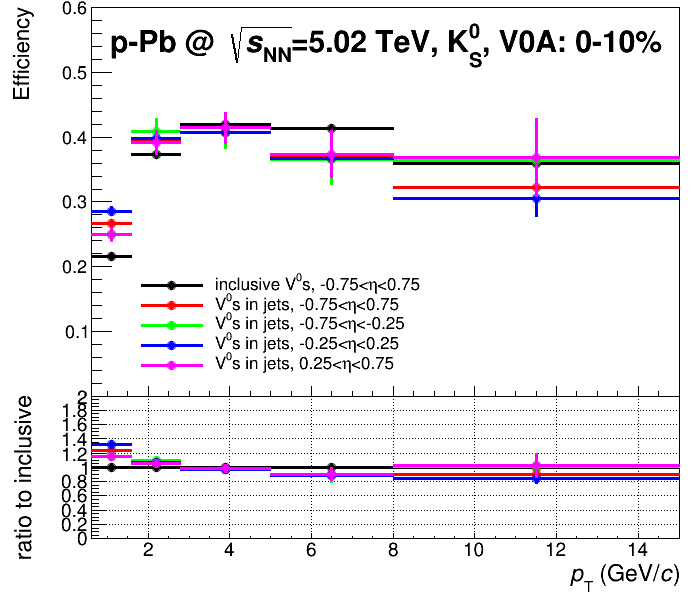
\includegraphics[width=.32\textwidth]{c05EffJetV0sMC/cKa_EffiJetEta_V0A_000_010}
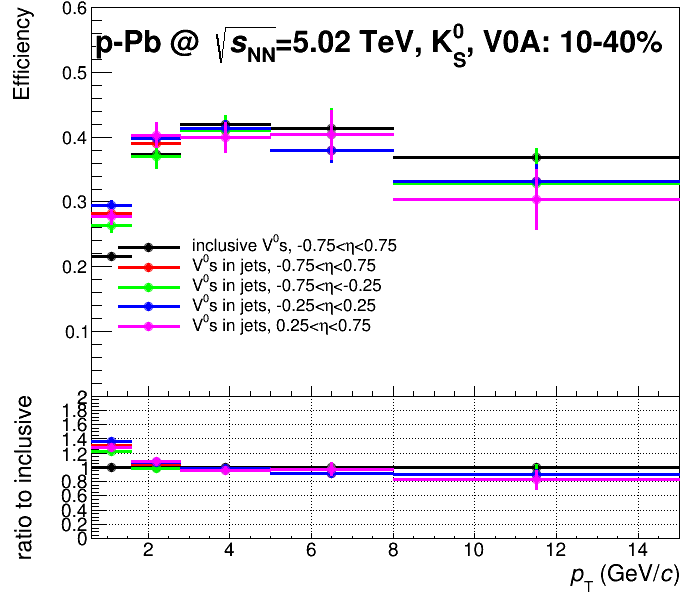
\includegraphics[width=.32\textwidth]{c05EffJetV0sMC/cKa_EffiJetEta_V0A_010_040}
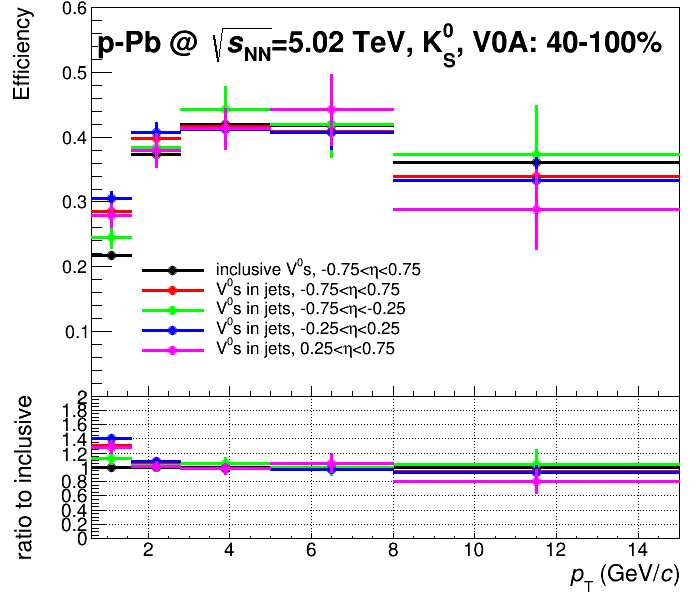
\includegraphics[width=.32\textwidth]{c05EffJetV0sMC/cKa_EffiJetEta_V0A_040_100}
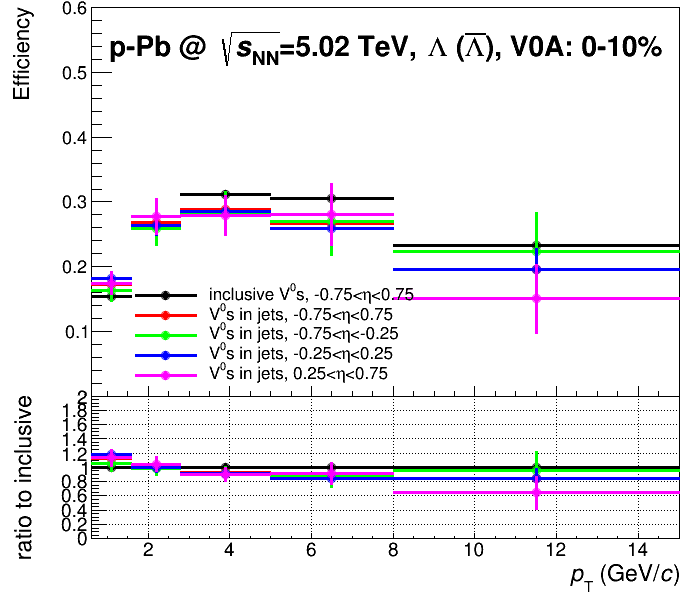
\includegraphics[width=.32\textwidth]{c05EffJetV0sMC/cLa_EffiJetEta_V0A_000_010}
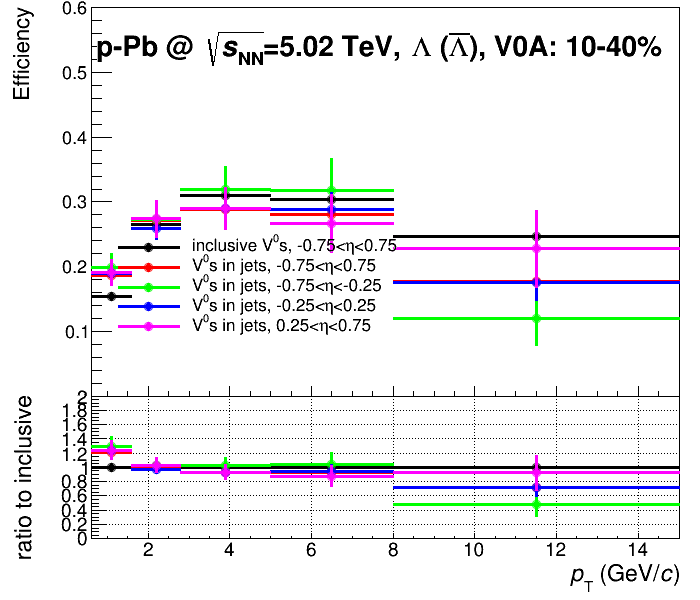
\includegraphics[width=.32\textwidth]{c05EffJetV0sMC/cLa_EffiJetEta_V0A_010_040}
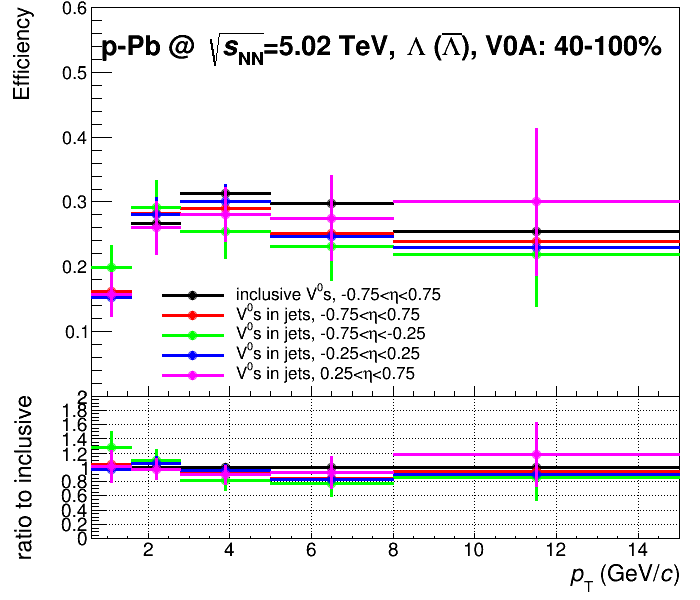
\includegraphics[width=.32\textwidth]{c05EffJetV0sMC/cLa_EffiJetEta_V0A_040_100}
\caption{Efficiency of $\Vzeros$ in jets as a function of $\pT$
         in three event multiplicity bins in simulations.
         The results are obtained in $\pT^{\rm jet}>10~\GeVc$.}
\label{fig:c05EffiJetV0sMC}
\end{center}
\end{figure}

Figure~\ref{fig:c05EffiJetV0sMC} shows the efficiency of $\Vzeros$ with jets
in $\pT>10~\GeVc$.
The results are compared with those of the inclusive $\Vzeros$ as well as
the those obtained in three sub-$\eta$ bins.
In general, the efficinecy of $\Vzeros$ in jets is $\sim 20\%$ higher than
that of inclusive $\Vzeros$ in low $\pT$ region.
At high $\pT$, the efficiency of $\Vzeros$ in jets is consistent with
the efficiency of inclusive $\Vzeros$.
To deeply handle the efficiency correction of the JC and OC $\Vzeros$,
one has to understand the reason for the increasing of the efficiency
JC $\Vzeros$ w.~r.~t. that of inclusive $\Vzeros$ in the low $\pT$ region.

\subsubsection{$\eta$ modified $\Vzero$ efficiency}
\label{sec:c05ScaledV0Effi}

\begin{figure}[htb]
\begin{center}
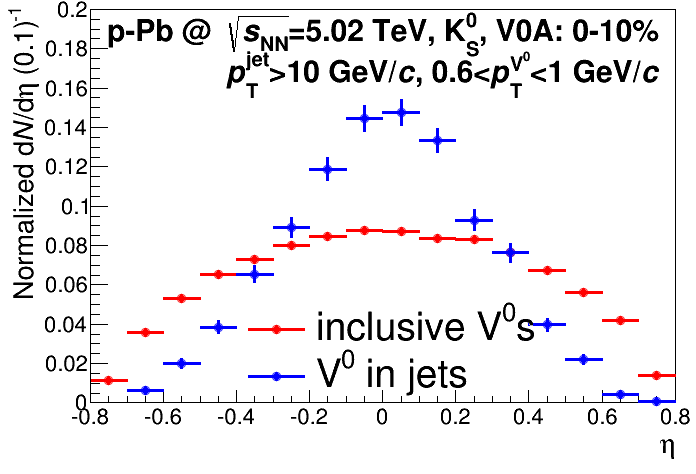
\includegraphics[width=.48\textwidth]{c05EffiV0Eta/cSpectra.png}
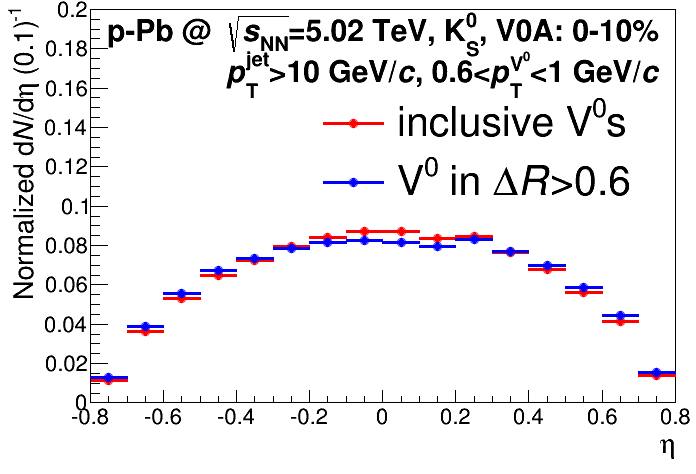
\includegraphics[width=.48\textwidth]{c05EffiV0Eta/cSpectra_OC}
\caption{Normalized $\eta$ distriubtion of $\Kshort$ in jets (left)
         and OC $\Kshort$ with $\Delta R>0.6$ (right) in data.
         The results are compared to the $\eta$ distriubtion of 
         inclusive and $\Kshort$.}
\label{fig:c05EffiJetV0Wgt}
\end{center}
\end{figure}

\begin{figure}[htb]
\begin{center}
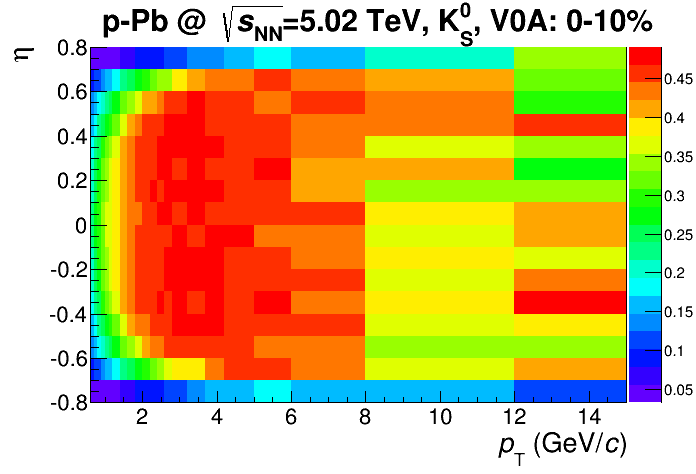
\includegraphics[width=.8\textwidth]{c05EffiV0Eta/cEfficiency_InclusiveV0}
\caption{2D efficiency of inclusive $\Vzeros$ as a function of $\pT$
         and $\eta$.}
\label{fig:c05EffiIncV02D}
\end{center}
\end{figure}

It has been shown that,
for the single $\Vzeros$, its efficiencies inside and outside the jets are
same~\cite{Kucera:AliPWGJE20140328}.
The difference between the efficiency of $\Vzeros$ in jets and
inclusive $\Vzeros$ is caused by the bias of the jet $\eta$ distribution.
Figure~\ref{fig:c05EffiJetV0Wgt} shows the normalized $\eta$ distribution
of JC $\Kshort$ candidates (left) and OC $\Kshort$ candidates
with $\Delta R_{\rm cut}>0.6$ (right) in $0.6<\pT<1~\GeVc$ in data.
The results are compared to the $\eta$ distribution of inclusive
and $\Kshort$ candidates.
The $\eta$ shape of JC $\Kshort$ candidates is modified by
the $\eta$ distribution of the jets.

As shown in figure~\ref{fig:c05EffiIncV02D},
the efficiency of inclusive $\Vzeros$ is non-uniform in $\eta$.
The integrated $\pT$-dependent $\Vzero$ efficiency can be treated as
weighted mean of the efficiency in the fine $\eta$ bins:
\begin{equation}\label{eq:c05WeightedEffi}
\varepsilon(\pT)=\frac{\sum_{\pT}r(\pT,\eta)}
                      {\sum_{\pT}g(\pT,\eta)}
 =\sum_{\pT}w(\pT,\eta)\varepsilon(\pT,\eta),
\end{equation}
where:
\begin{itemize}
\item $r(\pT,\eta)$ and $g(\pT,\eta)$ are the number of reconstructed and
      generated particles in each fine $\pT-\eta$ bin, respectively;
\item $w(\pT,\eta)=g(\pT,\eta)/\sum_{\pT}g(\pT,\eta)$ is the weight in the
      fine $\pT-\eta$ bins;
\item $\varepsilon(\pT,\eta)=r(\pT,\eta)/g(\pT,\eta)$ is the efficiency
      in the fine $\pT-\eta$ bins.
\end{itemize}
According to eq.~(\ref{eq:c05WeightedEffi}),
the bin has the larger counts will contribute the higher weight in the
integrated efficiency.
As show in the left panel of figure~\ref{fig:c05EffiJetV0Wgt},
the bin towards to $\eta=0$ in JC $\Vzero$ $\eta$ distribution has the
larger contribution in the integrated efficiency than that in the $\eta$
distribution of inclusive $\Vzeros$.
Due to the differential efficiency of $\Vzeros$ in the fine $\eta$ bin
towards to $\eta=0$ is higher than other,
it makes the increasing of the JC $\Vzero$ efficiency w.~r.~t. that of
the inclusive $\Vzeros$ in the low $\pT$
as shown in figure~\ref{fig:c05EffiJetV0sMC}.

To define the efficiency of the JC and OC $\Vzeros$ more precisely,
a scaling approach based on choosing a reference fine $\eta$ bin in data is
proposed~\cite{Zimmermann:AliPWGJE20140411}.
In this approach, the efficiency of JC and OC $\Vzeros$ in data is
calculated as:
\begin{equation}\label{eq:c05CorrEff}
\varepsilon_{\rm RD}(\pT)=
\frac{\sum_{\eta}n(\pT,\eta)}
     {\sum_{\eta}n(\pT,\eta)/\varepsilon_{\rm MC}(\pT,\eta)},
\end{equation}
where, $n(\pT,\eta)$ is the number of reconstructed $\Vzeros$ in the give
$\pT-\eta$ bin in data and $/\varepsilon_{\rm MC}(\pT,\eta)$ is the 2D
efficiency of inclusive $\Vzeros$ obtained in MC.
The basic consideration for this formula is according to the
efficiency of single $\Vzeros$ (either inside jets or outside jets) are the
same and it is described by the efficiency of the inclusive $\Vzeros$ in the
fine $\pT-\eta$ bins in MC.
The numerator are the reconstructed number of $\Vzeros$ in data,
while the denominator corresponds to the number of generated $\Vzeros$ in data.
In this case, the formula eq.~(\ref{eq:c05CorrEff}) can not only be used to
calculate the efficiency of the JC and OC $\Vzeros$ but also be used to
correct the efficiency of inclusive $\Vzeros$ as well as the efficiency
of NJ $\Vzeros$.

As discussed in section~\ref{sec:c03AnaStrategy} and
section~\ref{sec:c05V0EffiMC},
the interpolated bin counting fit results in data and MC have to be
subtracted in the term of $n(\pT,\eta)$ and the numerator
in the term of $\varepsilon_{\rm MC}(\pT,\eta)$ in eq.~(\ref{eq:c05CorrEff}),
respectively.
But due to the restriction of the statistics,
is it hard to make the stable bin counting fit in the side bands
in the fine $\pT-\eta$ bins in both data and MC.
In the implementation, we assume the bin counting ratio $R_{\rm Cbin}$,
which defined in eq.~(\ref{eq:c03CbinR}),
is independent on $\eta$ in both data and
MC (the uncertainty introduced by this assumption will
be discussed in section~\ref{sec:c06SystSingleV0s}).
And the efficiency calculation in this analysis is modified as:
\begin{equation}\label{eq:c05CorrEffImp}
\varepsilon_{\rm RD}(\pT)=
\frac{f_{\rm Cbin}^{\rm MC}(\pT)\cdot\sum_{\eta}n(\pT,\eta)}
     {\sum_{\eta}n(\pT,\eta)/\varepsilon_{\rm MC}(\pT,\eta)},
\end{equation}
where $f_{\rm Cbin}^{\rm MC}(\pT)=
       R_{\rm Cbin}^{\rm MC}(\pT)/(1+R_{\rm Cbin}^{\rm MC}(\pT))$,
$R_{\rm Cbin}^{\rm MC}(\pT)$ is the $\pT$-dependent bin counting ratio
in MC as show in the right panel of figure~\ref{fig:c03CbinRatio}.
Then in eq.~(\ref{eq:c05CorrEffImp}) the term of $n(\pT,\eta)$ and the
numerator in the term of $\varepsilon_{\rm MC}(\pT,\eta)$ now correspond to
the number of $\Vzero$ candidates (without the bin counting subtraction) in
each fine $\pT-\eta$ bin.

\begin{figure}[htb]
\begin{center}
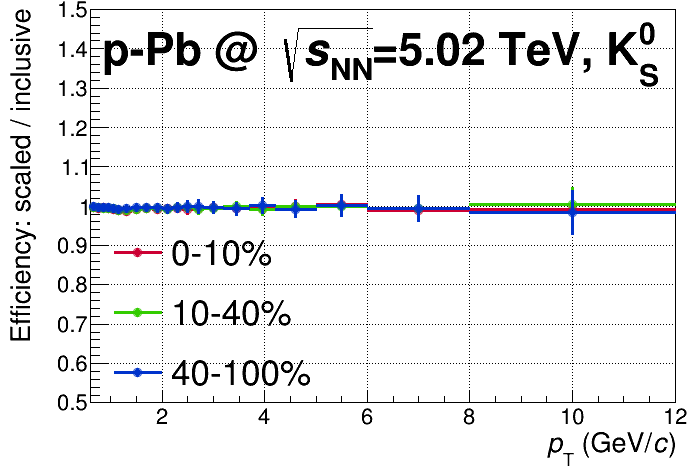
\includegraphics[width=.32\textwidth]{c05ScaledV0Effi/cCompEffIncl_Kshort}
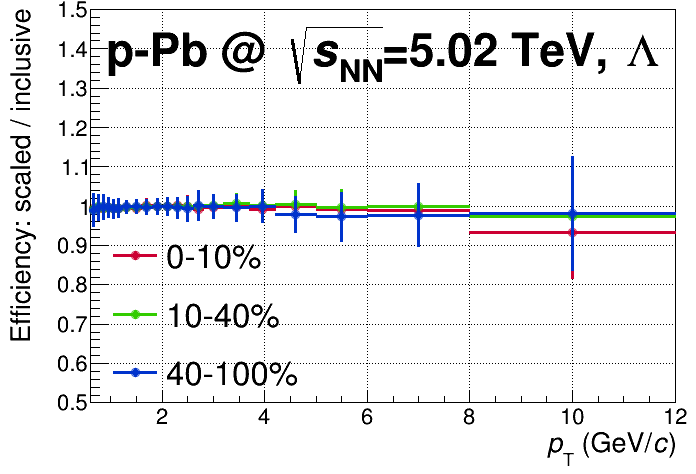
\includegraphics[width=.32\textwidth]{c05ScaledV0Effi/cCompEffIncl_Lambda}
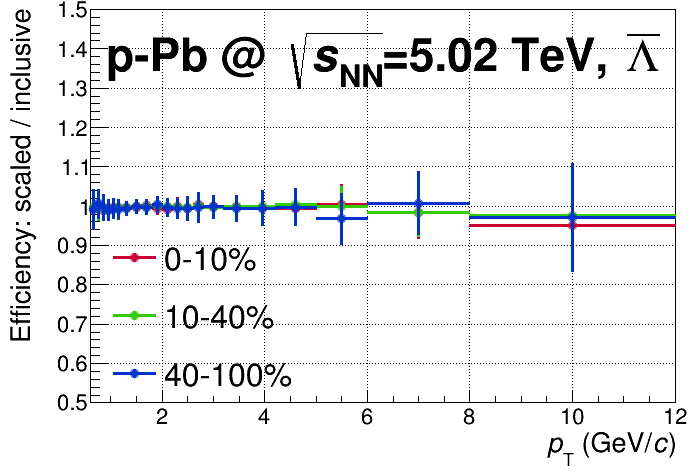
\includegraphics[width=.32\textwidth]{c05ScaledV0Effi/cCompEffIncl_AntiLa}
\caption{The ratio between the scaled inclusive $\Vzero$ efficiency
         calculated by using eq.~(\ref{eq:c05CorrEffImp}) and the
         inclusive $\Vzero$ efficiency in MC as shown
         in figure~\ref{fig:c05EffiIncV0s}.}
\label{fig:c05CompScaledEff}
\end{center}
\end{figure}

\begin{figure}[htb]
\begin{center}
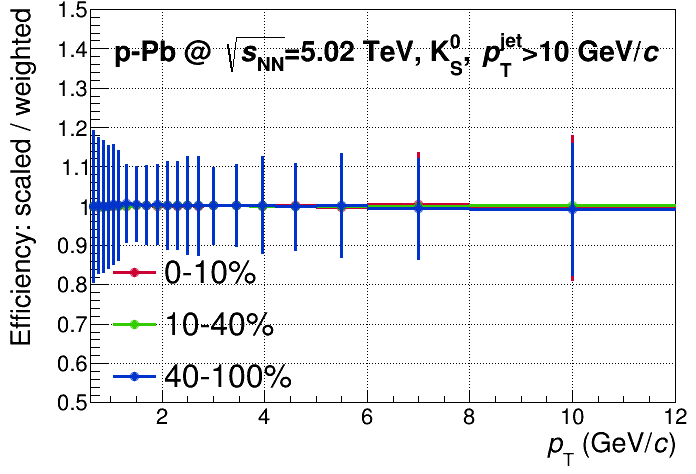
\includegraphics[width=.32\textwidth]{c05ScaledV0Effi/cCompEffWght_Kshort_PtJ10_JC}
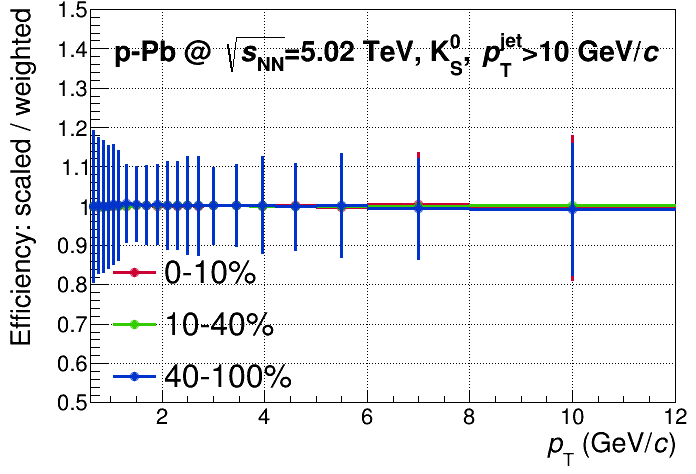
\includegraphics[width=.32\textwidth]{c05ScaledV0Effi/cCompEffWght_Kshort_PtJ10_JC}
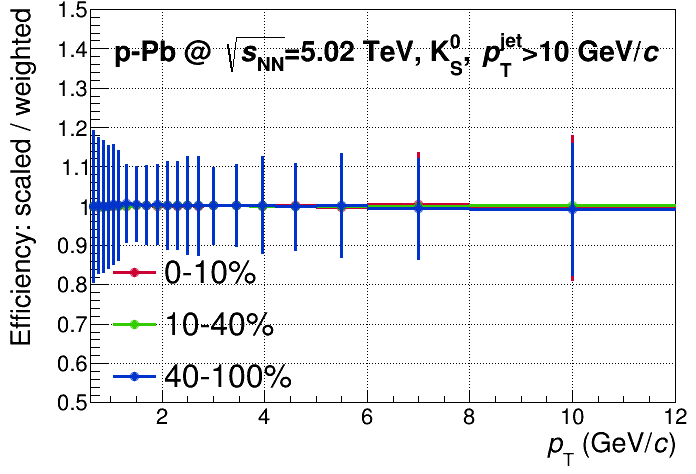
\includegraphics[width=.32\textwidth]{c05ScaledV0Effi/cCompEffWght_Kshort_PtJ10_JC}
\caption{The ratio between the scaled JC $\Vzero$ efficiency calculated by
         using eq.~(\ref{eq:c05CorrEffImp}) and the JC $\Vzero$ efficiency
         calculated by the weighting approach described in
         appendix~\ref{sec:a01WghtV0Effi}.
         The results are obtained in $\pT^{\rm jet}>10~\GeVc$.}
\label{fig:c05CompScaledWghtPtJ10JC}
\end{center}
\end{figure}

\begin{figure}[htb]
\begin{center}
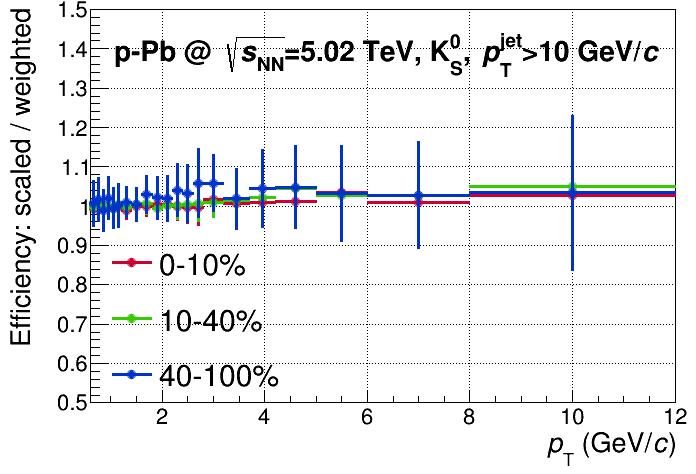
\includegraphics[width=.32\textwidth]{c05ScaledV0Effi/cCompEffWght_Kshort_PtJ10_OC06}
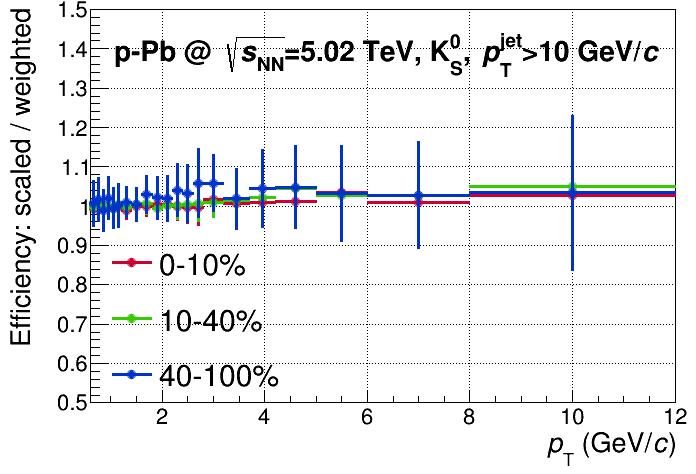
\includegraphics[width=.32\textwidth]{c05ScaledV0Effi/cCompEffWght_Kshort_PtJ10_OC06}
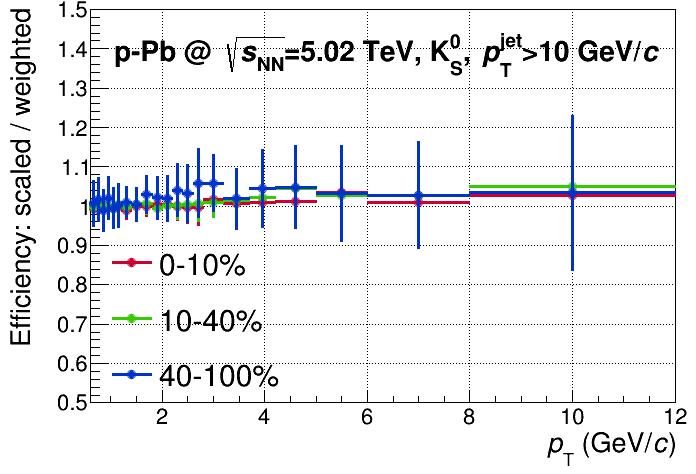
\includegraphics[width=.32\textwidth]{c05ScaledV0Effi/cCompEffWght_Kshort_PtJ10_OC06}
\caption{The ratio between the scaled OC $\Vzero$ efficiency calculated by
         using eq.~(\ref{eq:c05CorrEffImp}) and the OC $\Vzero$ efficiency
         calculated by the weighting approach described in
         appendix~\ref{sec:a01WghtV0Effi}.
         The results are obtained in $\pT^{\rm jet}>10~\GeVc$.
         The OC $\Vzeros$ are obtained with $\Delta R_{\rm cut}=0.6$.}
\label{fig:c05CompScaledWghtPtJ10OC06}
\end{center}
\end{figure}

\begin{figure}[htb]
\begin{center}
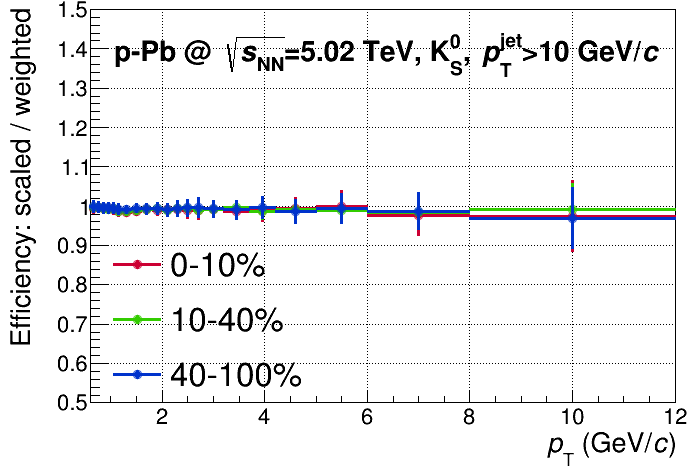
\includegraphics[width=.32\textwidth]{c05ScaledV0Effi/cCompEffWght_Kshort_PtJ05_NJ}
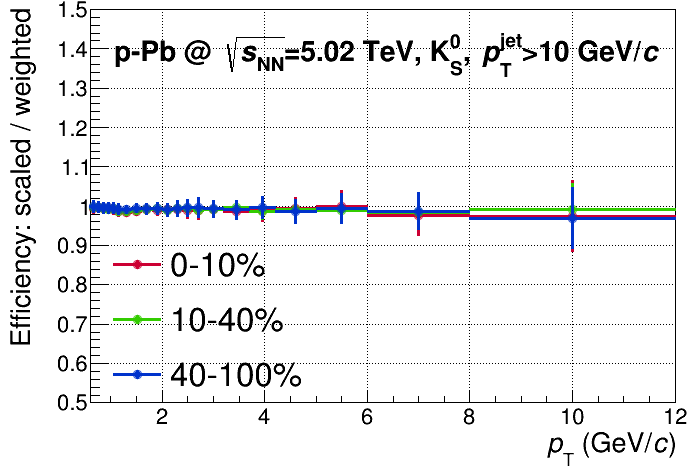
\includegraphics[width=.32\textwidth]{c05ScaledV0Effi/cCompEffWght_Kshort_PtJ05_NJ}
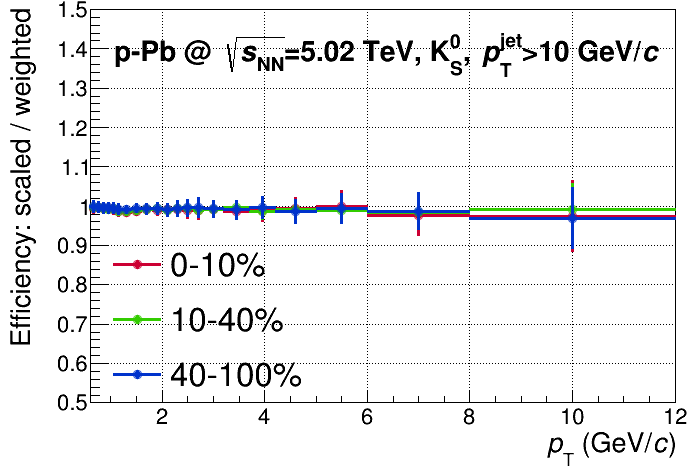
\includegraphics[width=.32\textwidth]{c05ScaledV0Effi/cCompEffWght_Kshort_PtJ05_NJ}
\caption{The ratio between the scaled NJ $\Vzero$ efficiency calculated by
         using eq.~(\ref{eq:c05CorrEffImp}) and the NJ $\Vzero$ efficiency
         calculated by the weighting approach described in
         appendix~\ref{sec:a01WghtV0Effi}.}
\label{fig:c05CompScaledWghtPtJ10NJ}
\end{center}
\end{figure}

Figure~\ref{fig:c05CompScaledEff} shows the ratio of the inclusive $\Vzero$
efficiency calculated by the scaling approach according
to eq.~(\ref{eq:c05CorrEffImp}) and the efficiency of
inclusive $\Vzeros$ in MC which is shown in figure~\ref{fig:c05EffiIncV0s}
in three event centrality bins.
In general, the discrepancy between the efficiency calculated by this
two approaches is $\sim 1\%$.
The ratio of the efficiency of the JC, OC and NJ $\Vzeros$ calculated by the
scaling approaching and those calculated by a weighting approach (introduced
in appendix~\ref{sec:a01WghtV0Effi}) are shown in
figure~\ref{fig:c05CompScaledWghtPtJ10JC},
figure~\ref{fig:c05CompScaledWghtPtJ10OC06} and
figure~\ref{fig:c05CompScaledWghtPtJ10NJ}, respectively.
The maximum deviation between the efficiencies obtained by these two methods
is $\sim 5\%$.

Please note that,
the error bars on the ratios in the figures are the statistic uncertainty
propagated by ROOT.
And indeed, the uncertainty propagation in the efficiency calculation is not
straight forward.
The details for the uncertainty will be discussed
in section~\ref{sec:c06StatErrors}.

\subsection{Underlying background subtraction}\label{sec:c05NormV0s}

The corrected spectrum of any type of $\Vzeros$
is given by:
\begin{equation}\label{eq:c05EffiCorrV0s}
\frac{{\rm d}N}{{\rm d}\pT}=m(\pT)/\varepsilon_{\rm RD}(\pT),
\end{equation}
where $m(\pT)$ is number of $\Vzeros$ in the given $\pT$ bin after the
bin counting subtraction,
$\varepsilon_{\rm RD}(\pT)$ is the corrected $\Vzero$ efficiency by the
scaling procedure in eq.~(\ref{eq:c05CorrEffImp}).

Since the UE $\Vzeros$ are used to estimate the UE background per acceptance
area density inside the jet cone,
to obtain the $\Vzeros$ produced in jets ({\bf JE $\mathbf\Vzeros$}),
we normalize the yields of both JC and UE $\Vzeros$ to the
per-event acceptance area unit to subtract the UE $\Vzero$ background:
\begin{equation}\label{eq:c05NormV0sJE}
\frac{{\rm d}M_{\rm JE}}{{\rm d}\pT}=
\frac{{\rm d}M_{\rm JC}}{{\rm d}\pT}-\frac{{\rm d}M_{\rm UE}}{{\rm d}\pT},
\end{equation}
where, for the JC and UE $\Vzeros$ the term ${\rm d}M/{\rm d}\pT$ is given by:
\begin{equation}\label{eq:c05NormCorrV0s}
\frac{{\rm d}M_{\rm JC/UE}}{{\rm d}\pT}=
\frac{1}{N_{\rm JC/UE}^{\rm ev}}\times\frac{1}{\Delta\eta\Delta\phi}\times
\frac{{\rm d}N_{\rm JC/UE}}{{\rm d}\pT}.
\end{equation}
In eq.~(\ref{eq:c05NormCorrV0s}),
the term ${\rm d}N_{\rm JC/UE}/{\rm d}\pT$ is the corrected JC or
UE $\Vzero$ spectrum defined in eq.~(\ref{eq:c05EffiCorrV0s}),
$N_{\rm JC/UE}^{\rm ev}$ is the corresponding number of JC or UE events and
$\Delta\eta\times\Delta\phi$ is the per-event acceptance area for
the JC or UE $\Vzeros$.

For the JC or OC $\Vzeros$, since they are obtained in the events have at
least one selected jet in $\pT^{\rm jet}>\pT^{\min}$~\footnote{As discussed
in section~\ref{sec:c05EstiV0sUE},
there are two set of values are chosen
for the $\pT^{\min}$: $\pT^{\min}=10~\GeVc$ and $\pT^{\min}=20~\GeVc$ in
this analysis.},
the $N_{\rm JC/OC}^{\rm ev}$ for the JC or OC $\Vzeros$ is number of events
with at least one selected jet in  $\pT^{\rm jet}>\pT^{\min}$.
For NJ $\Vzeros$, the $N_{\rm NJ}^{\rm ev}$ is the number of events have
no jet in $\pT>5~\GeVc$.

According to the definition,
the per-event acceptance area for NJ $\Vzeros$ is equal to the
acceptance of the inclusive $\Vzero$ define in section~\ref{sec:c05DefAcc}:
\begin{equation}
[\Delta\eta\times\Delta\phi]_{\rm NJ}=2\times 0.75\times 2\pi.
\end{equation}

Concerning the calculation of the per-event acceptance area for the JC or
OC $\Vzeros$ ($[\Delta\eta\times\Delta\phi]_{\rm JC/OC}$),
the following MC approach is adopted:
\begin{enumerate}
\item generate the a given number of testing particles with the
      randomized $\eta$ and $\phi$ in the $\Vzero$ acceptance according to the
      $\eta-\phi$ distribution of the the JC or OC $\Vzero$ candidates (in this
      analysis, $10^{3}$ testing particles are generated in each event),
\item match the testing particles to the jets in each given event
      and count the numbers of the testing particles inside and outside
      the jet cones;
\item the ratio of the number of the JC/OC particles and the number of
      total generated particles gives the fraction of acceptance for
      the JC/OC $\Vzeros$ in the given event;
\item the final acceptance correction factor of JC/OC $\Vzeros$ is given
      by the average of the event-by-event acceptance fraction.
\end{enumerate}

\begin{figure}[htb]
\begin{center}
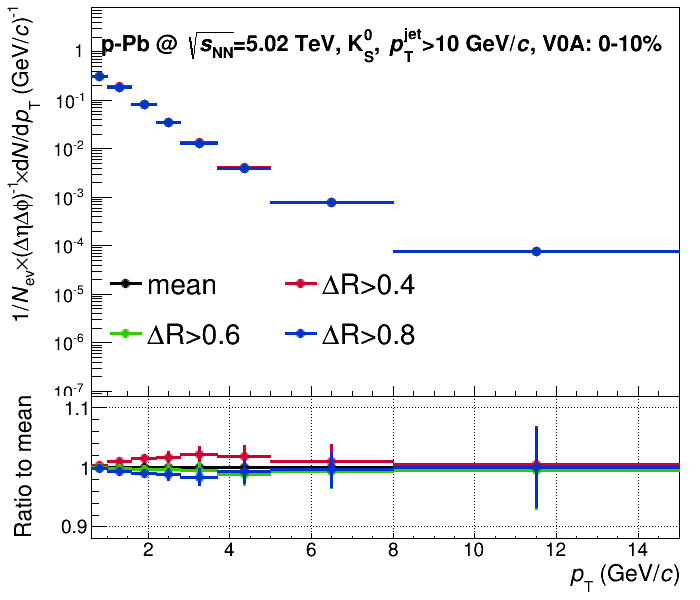
\includegraphics[width=.32\textwidth]{c05Results/cKshort_Comp_OC_JE_V0A_000_010_PtJ10}
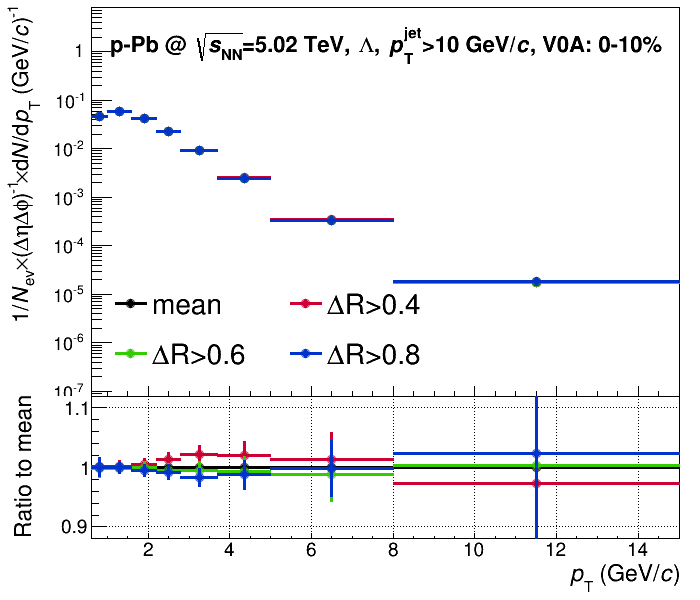
\includegraphics[width=.32\textwidth]{c05Results/cLambda_Comp_OC_JE_V0A_000_010_PtJ10}
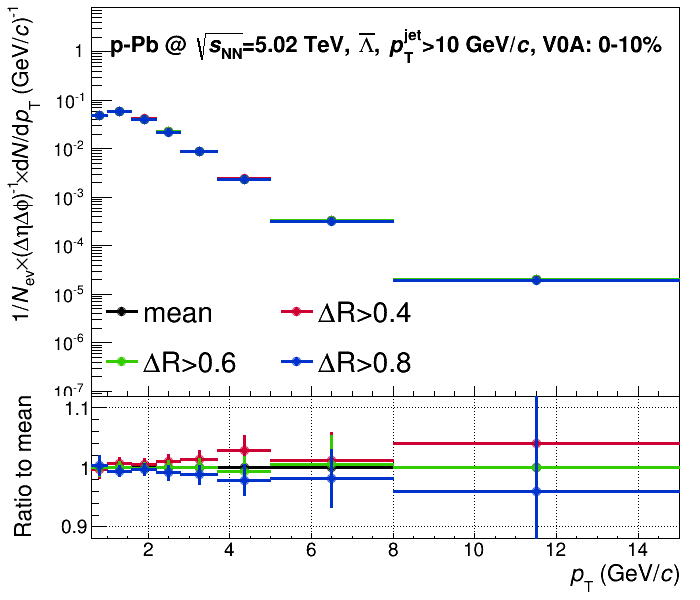
\includegraphics[width=.32\textwidth]{c05Results/cAntiLa_Comp_OC_JE_V0A_000_010_PtJ10}
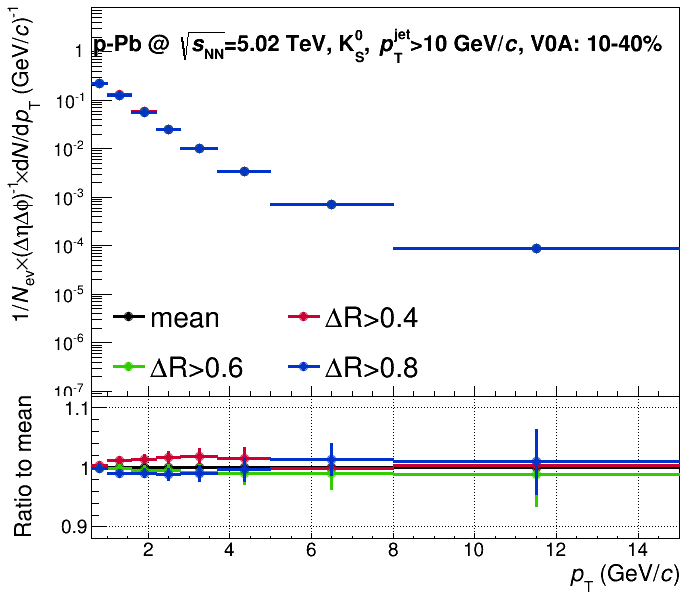
\includegraphics[width=.32\textwidth]{c05Results/cKshort_Comp_OC_JE_V0A_010_040_PtJ10}
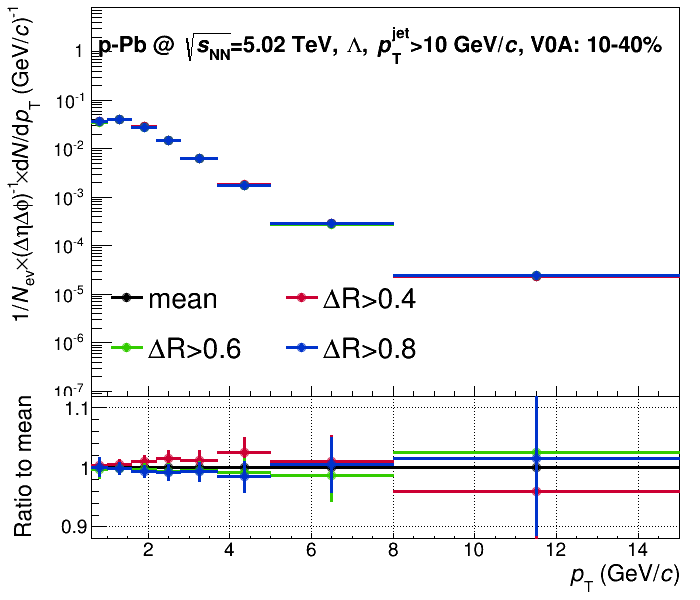
\includegraphics[width=.32\textwidth]{c05Results/cLambda_Comp_OC_JE_V0A_010_040_PtJ10}
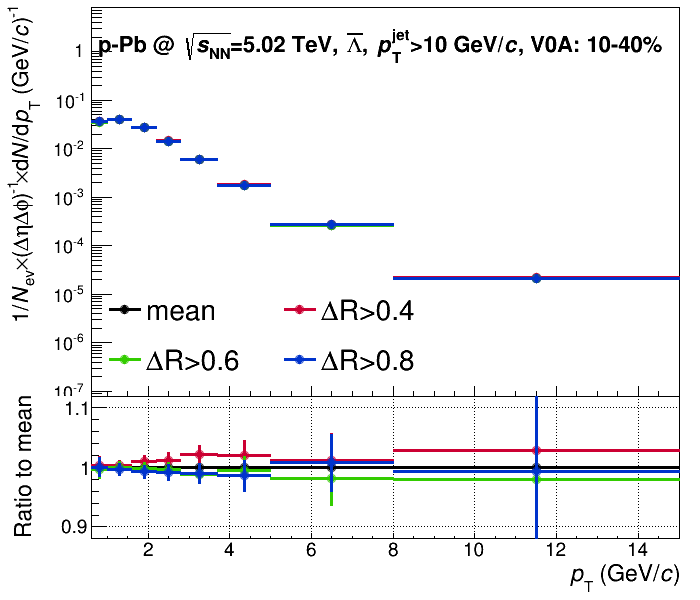
\includegraphics[width=.32\textwidth]{c05Results/cAntiLa_Comp_OC_JE_V0A_010_040_PtJ10}
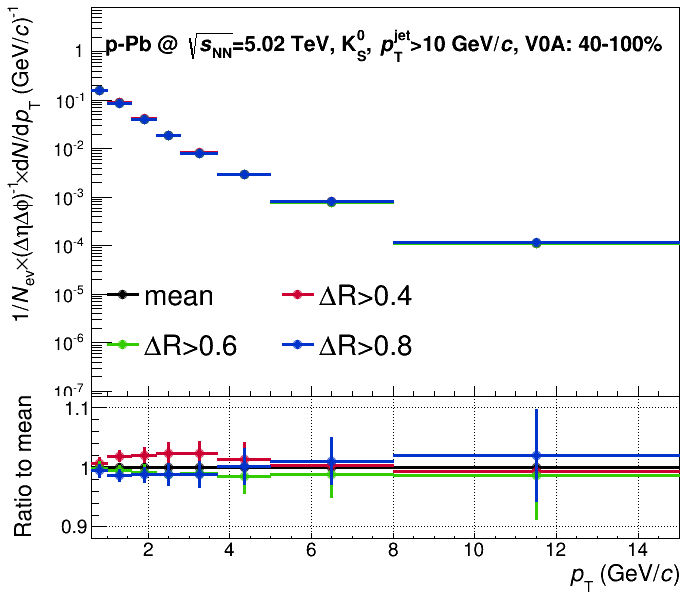
\includegraphics[width=.32\textwidth]{c05Results/cKshort_Comp_OC_JE_V0A_040_100_PtJ10}
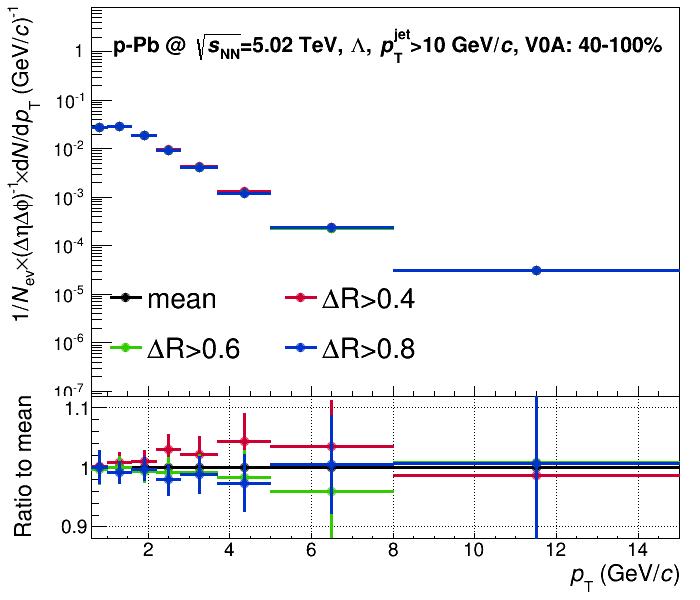
\includegraphics[width=.32\textwidth]{c05Results/cLambda_Comp_OC_JE_V0A_040_100_PtJ10}
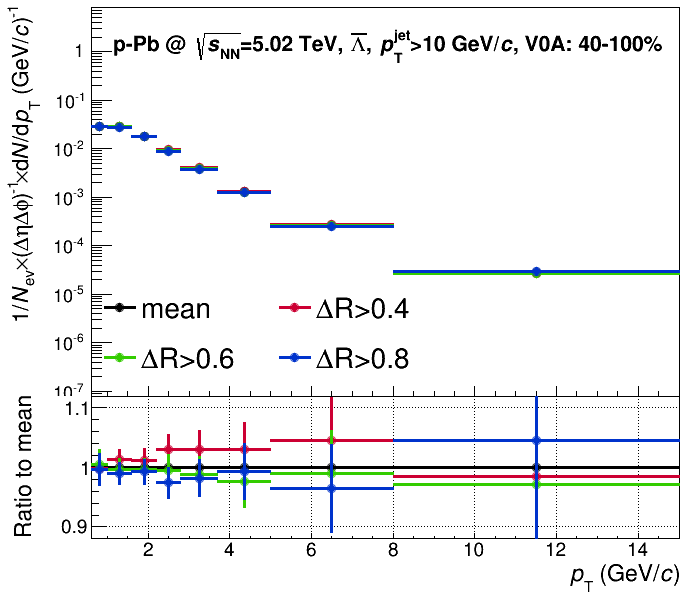
\includegraphics[width=.32\textwidth]{c05Results/cAntiLa_Comp_OC_JE_V0A_040_100_PtJ10}
\caption{Normalized ${\rm OC}~\Vzeros$ with different $\Delta R$ in
         $\pT^{\rm jet}>10~\GeVc$.}
\label{fig:c05RestulsCompOCPtJ10}
\end{center}
\end{figure}

\begin{figure}[htb]
\begin{center}
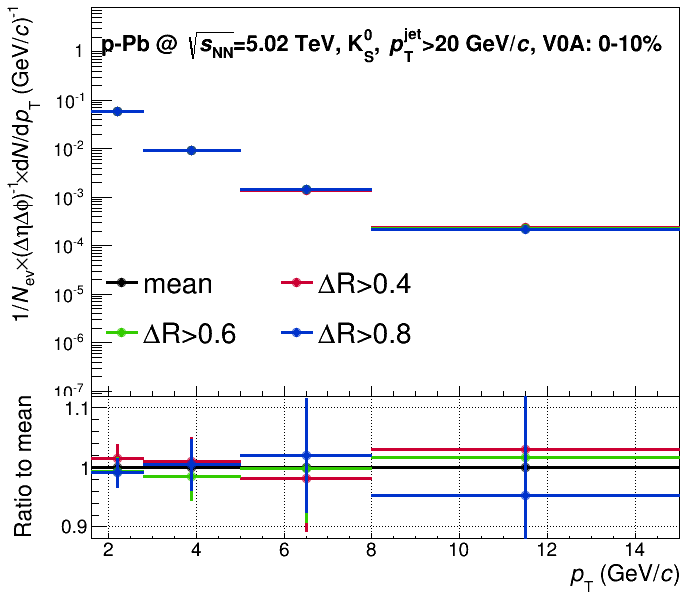
\includegraphics[width=.32\textwidth]{c05Results/cKshort_Comp_OC_JE_V0A_000_010_PtJ20}
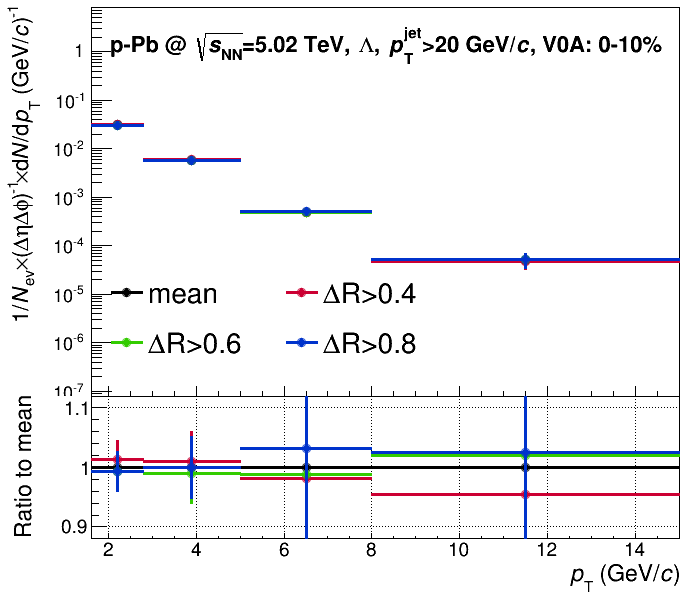
\includegraphics[width=.32\textwidth]{c05Results/cLambda_Comp_OC_JE_V0A_000_010_PtJ20}
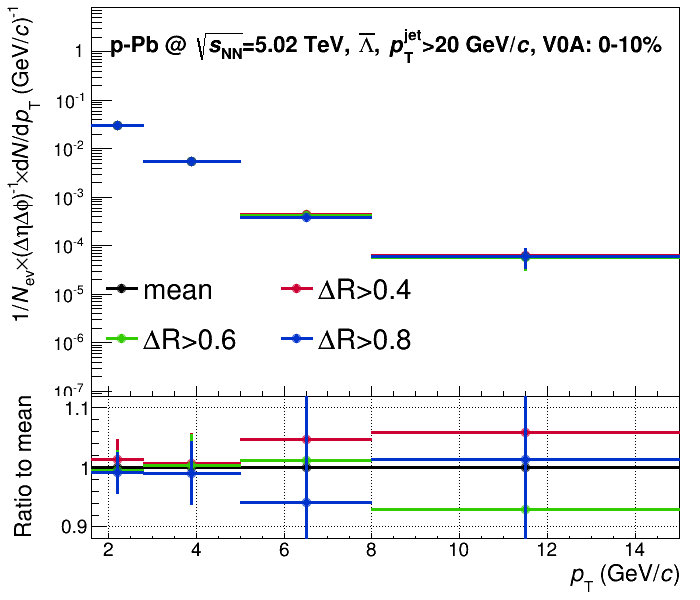
\includegraphics[width=.32\textwidth]{c05Results/cAntiLa_Comp_OC_JE_V0A_000_010_PtJ20}
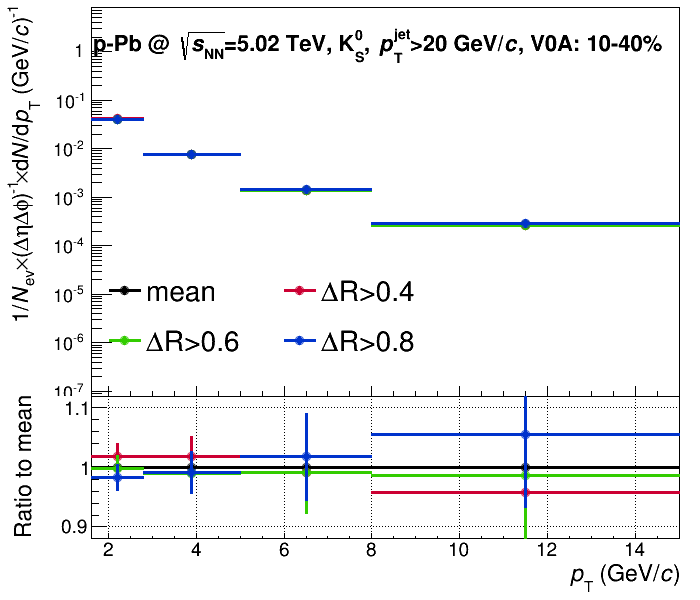
\includegraphics[width=.32\textwidth]{c05Results/cKshort_Comp_OC_JE_V0A_010_040_PtJ20}
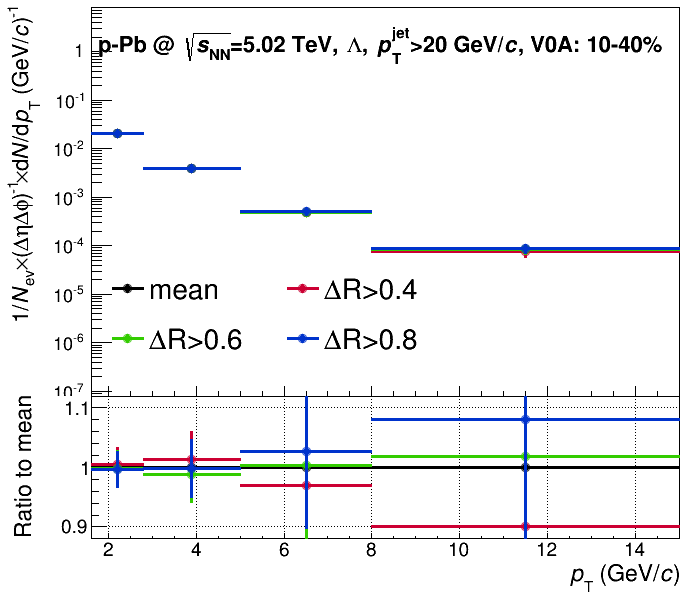
\includegraphics[width=.32\textwidth]{c05Results/cLambda_Comp_OC_JE_V0A_010_040_PtJ20}
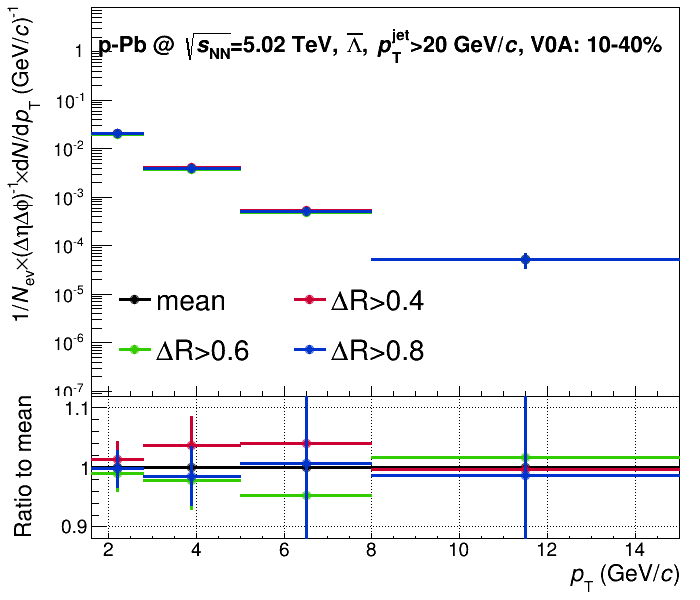
\includegraphics[width=.32\textwidth]{c05Results/cAntiLa_Comp_OC_JE_V0A_010_040_PtJ20}
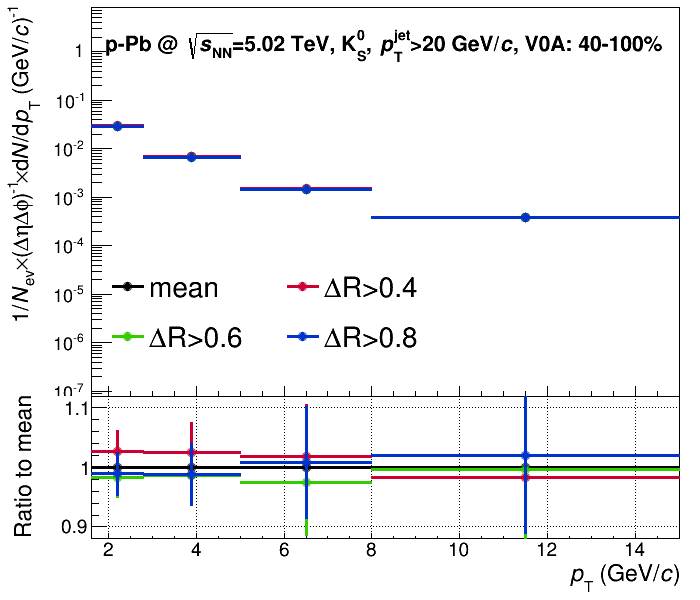
\includegraphics[width=.32\textwidth]{c05Results/cKshort_Comp_OC_JE_V0A_040_100_PtJ20}
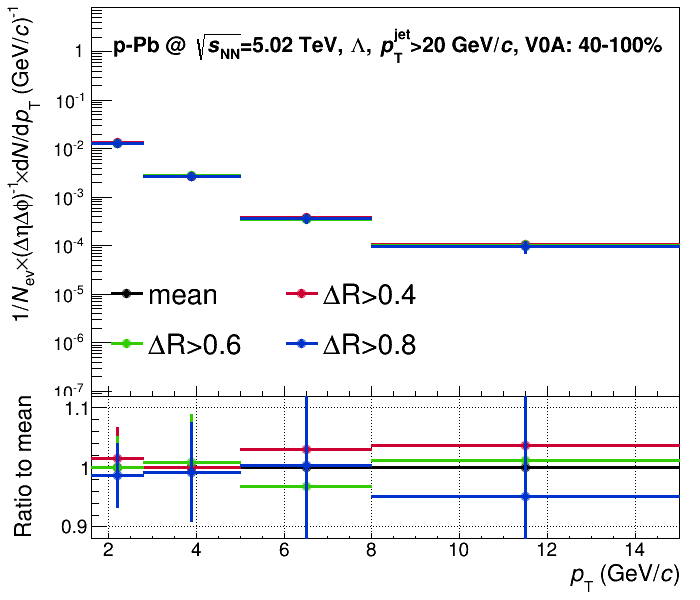
\includegraphics[width=.32\textwidth]{c05Results/cLambda_Comp_OC_JE_V0A_040_100_PtJ20}
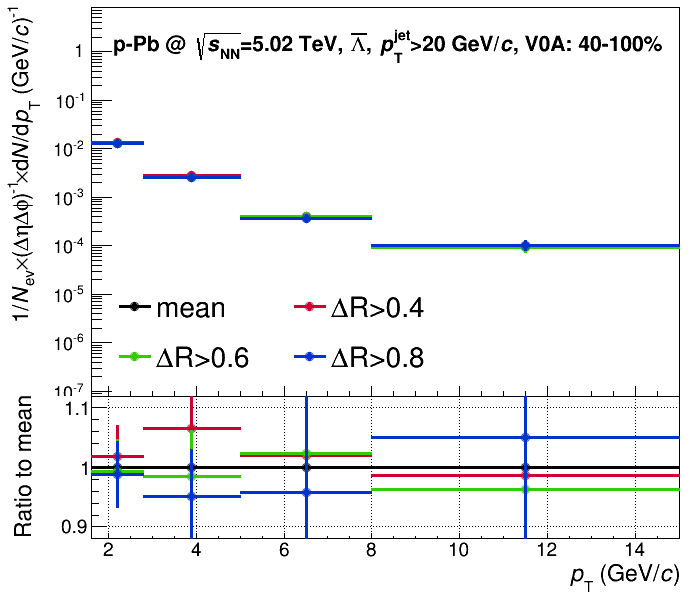
\includegraphics[width=.32\textwidth]{c05Results/cAntiLa_Comp_OC_JE_V0A_040_100_PtJ20}
\caption{Normalized ${\rm OC}~\Vzeros$ with different $\Delta R$
         in $\pT^{\rm jet}>20~\GeVc$.}
\label{fig:c05RestulsCompOCPtJ20}
\end{center}
\end{figure}


\subsection{Feeddown subtraction}

To obtain the final corrected spectra for $\Lambda$ and $\AntiLa$ the feeddown
components from $\Xi$ decays has to be subtracted.
The method used for the  feeddown subtraction for the inclusive $\Vzeros$
is introduced in~\cite{Ali2012:ana501}.
According to this method, the subtraction has to be applied before the
efficiency correction.

To apply the feeddown subtraction of the $\Vzeros$ in jets,
the following issues has to be considered:
\begin{itemize}
\item we have not measured the $\Xi$ produce inside jets yet;
\item the $\Vzeros$ produced inside jets are obtained by subtract the
      UE $\Vzeros$ from the JC $\Vzeros$ and the JC $\Vzeros$ are composed
      by the following four components:
      \begin{equation}\label{eq:c05CompsInJC}
      {\rm JC}={\rm JC}_{\rm H}+
               {\rm JC}_{\rm F}+{\rm UE}_{\rm H}+{\rm UE}_{\rm F},
      \end{equation}
      where,
      \begin{itemize}
      \item ${\rm JC}_{\rm H}~\Vzeros$
            is the primary $\Vzeros$ produced inside jets and
            they are what we are going to measured in this analysis;
      \item ${\rm JC}_{\rm F}~\Vzeros$
            is the feeddown $\Vzeros$ matched with the jets;
      \item ${\rm UE}_{\rm H}~\Vzeros$
            is the primary $\Vzeros$ in matched with the jets but
            from the underlying event;
      \item ${\rm UE}_{\rm F}$ is the feeddown $\Vzeros$ matched with jets
            but from the underlying event.
      \end{itemize}
\end{itemize}

Since the efficiency correction will not change the ratios of
${\rm JC}_{\rm H}~\Vzeros/{\rm JC}_{\rm F}~\Vzeros$ and
${\rm UE}_{\rm H}~\Vzeros/{\rm UE}_{\rm F}~\Vzeros$
in the JC $\Vzero$ component.
the following steps are used to subtract the feeddown contributions
for the $\Vzero$ produced inside jets:
\begin{enumerate}
\item apply the efficiency correction for both JC and UE $\Vzeros$ without
      the feeddown subtraction;
\item subtract the normalized UE component from the JC $\Vzeros$,
      in this procedure,
      the last two terms in eq.~{\ref{eq:c05CompsInJC}} are subtracted;
\item subtract the feeddown $\Vzeros$ matched with
      jets (${\rm JC}_{\rm F}~\Vzeros$) according to the estimated
      fedddown fraction.
\end{enumerate}

The uncertainty of this feeddown subtraction strategy will be
discussed in section~\ref{sec:c06SystFd}.

\begin{figure}[htb]
\begin{center}
\includegraphics[width=.32\textwidth]{c05Results/cKshort_Comp_JC_JE_V0A_000_010_PtJ10}
\includegraphics[width=.32\textwidth]{c05Results/cLambda_Comp_JC_JE_V0A_000_010_PtJ10}
\includegraphics[width=.32\textwidth]{c05Results/cAntiLa_Comp_JC_JE_V0A_000_010_PtJ10}
\includegraphics[width=.32\textwidth]{c05Results/cKshort_Comp_JC_JE_V0A_010_040_PtJ10}
\includegraphics[width=.32\textwidth]{c05Results/cLambda_Comp_JC_JE_V0A_010_040_PtJ10}
\includegraphics[width=.32\textwidth]{c05Results/cAntiLa_Comp_JC_JE_V0A_010_040_PtJ10}
\includegraphics[width=.32\textwidth]{c05Results/cKshort_Comp_JC_JE_V0A_040_100_PtJ10}
\includegraphics[width=.32\textwidth]{c05Results/cLambda_Comp_JC_JE_V0A_040_100_PtJ10}
\includegraphics[width=.32\textwidth]{c05Results/cAntiLa_Comp_JC_JE_V0A_040_100_PtJ10}
\caption{Normalized JC $\Vzeros$ and UE $\Vzeros$ in $\pT^{\rm jet}>10~\GeVc$,
         results are compared to the inclusive $\Vzeros$.}
\label{fig:c05RestulsCompJCPtJ10}
\end{center}
\end{figure}

\begin{figure}[htb]
\begin{center}
\includegraphics[width=.32\textwidth]{c05Results/cKshort_Comp_JC_JE_V0A_000_010_PtJ20}
\includegraphics[width=.32\textwidth]{c05Results/cLambda_Comp_JC_JE_V0A_000_010_PtJ20}
\includegraphics[width=.32\textwidth]{c05Results/cAntiLa_Comp_JC_JE_V0A_000_010_PtJ20}
\includegraphics[width=.32\textwidth]{c05Results/cKshort_Comp_JC_JE_V0A_010_040_PtJ20}
\includegraphics[width=.32\textwidth]{c05Results/cLambda_Comp_JC_JE_V0A_010_040_PtJ20}
\includegraphics[width=.32\textwidth]{c05Results/cAntiLa_Comp_JC_JE_V0A_010_040_PtJ20}
\includegraphics[width=.32\textwidth]{c05Results/cKshort_Comp_JC_JE_V0A_040_100_PtJ20}
\includegraphics[width=.32\textwidth]{c05Results/cLambda_Comp_JC_JE_V0A_040_100_PtJ20}
\includegraphics[width=.32\textwidth]{c05Results/cAntiLa_Comp_JC_JE_V0A_040_100_PtJ20}
\caption{Normalized JC $\Vzeros$ and UE $\Vzeros$ in $\pT^{\rm jet}>20~\GeVc$,
         results are compared to the inclusive $\Vzeros$.}
\label{fig:c05RestulsCompJCPtJ20}
\end{center}
\end{figure}

\subsection{Normalized results}
\label{sec:c05NormResults}

The normalized spectra of OC $\Vzeros$ are shown in
figure~\ref{fig:c05RestulsCompOCPtJ10} and
figure~\ref{fig:c05RestulsCompOCPtJ20} with $\pT^{\rm jet}>10~\GeVc$ and
$\pT^{\rm jet}>20~\GeVc$, respectively.
The charged jets are reconstructed with $R_{\rm jet}=0.4$.
In general, the difference between the OC $\Vzeros$ with
different $\Delta R_{\rm cut}$ is small ($\sim 2\%$).
With smaller $\Delta R_{\rm cut}$ (e.g. $\Delta R_{\rm cut}=0.4$),
the correlations between the OC component and JC $\Vzeros$ is stronger.
And its normalized spectrum is systematically higher
than the ones with  larger $\Delta R_{\rm cut}$.


The normalized $\pT$ spectra for different type of $\Vzeros$ are
compared in figure~\ref{fig:c05RestulsCompJCPtJ10} and
figure~\ref{fig:c05RestulsCompJCPtJ20}
with $\pT^{\rm jet}>10~\GeVc$ and $\pT^{\rm jet}>20~\GeVc$, respectively.
As expected, the spectra of OC and NJ $\Vzeros$ are very close to the that
of the inclusive $\Vzeros$ in the low $\pT$ region since the
inclusive $\Vzero$ production is dominated by the $\Vzeros$ from
the underlying events.
In the high $\pT$ region,
the spectra of OC $\Vzeros$ is harder than that of the inclusive $\Vzeros$
and the spectra of NJ $\Vzeros$ is softer than the inclusive ones.
As mentioned in section~\ref{sec:c05EstiV0sUE} the OC $\Vzeros$ may include
the component come from the jets excluded by the jet selection.
And the contribution from the $\Vzeros$ produced inside the jets are
highly suppressed in the sample of the NJ $\Vzeros$ and it makes its
spectrum is softer than that of the inclusive $\Vzeros$.
Despite this difference, the spectra of both the OC and NJ $\Vzeros$
are much softer than that of the JC $\Vzeros$ (as expected,
the high $\pT$ $\Vzero$ are mainly contributed by the jet production),
the uncertainty introduced by the UE $\Vzero$ subtraction should be
small in the high $\pT$ region.
